% Created by tikzDevice version 0.11 on 2018-09-26 14:31:12
% !TEX encoding = UTF-8 Unicode
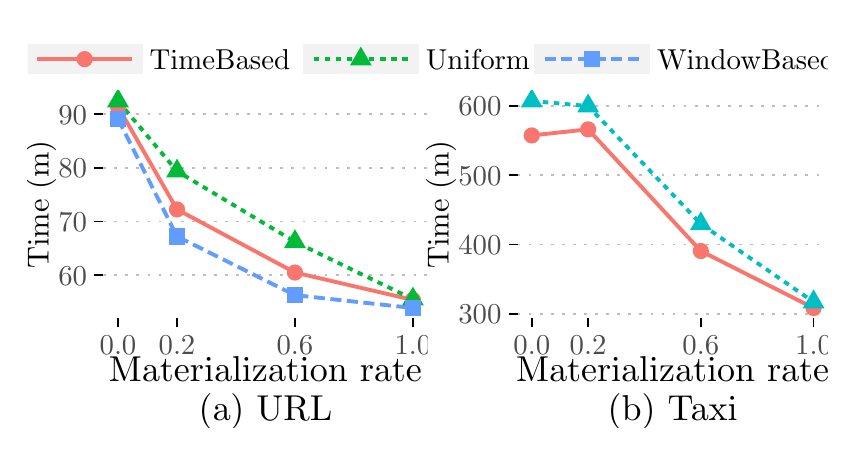
\begin{tikzpicture}[x=1pt,y=1pt]
\definecolor{fillColor}{RGB}{255,255,255}
\path[use as bounding box,fill=fillColor,fill opacity=0.00] (0,0) rectangle (289.08,144.54);
\begin{scope}
\path[clip] (  0.00,  0.00) rectangle (289.08,144.54);
\definecolor{fillColor}{RGB}{255,255,255}

\path[fill=fillColor] (-10.79,121.78) rectangle (299.87,144.54);
\end{scope}
\begin{scope}
\path[clip] (  0.00,  0.00) rectangle (289.08,144.54);
\definecolor{drawColor}{RGB}{255,255,255}
\definecolor{fillColor}{gray}{0.95}

\path[draw=drawColor,line width= 0.6pt,line join=round,line cap=round,fill=fillColor] ( -0.76,127.47) rectangle ( 41.92,138.85);
\end{scope}
\begin{scope}
\path[clip] (  0.00,  0.00) rectangle (289.08,144.54);
\definecolor{drawColor}{RGB}{248,118,109}

\path[draw=drawColor,line width= 1.4pt,line join=round] (  3.50,133.16) -- ( 37.65,133.16);
\end{scope}
\begin{scope}
\path[clip] (  0.00,  0.00) rectangle (289.08,144.54);
\definecolor{fillColor}{RGB}{248,118,109}

\path[fill=fillColor] ( 20.58,133.16) circle (  2.93);
\end{scope}
\begin{scope}
\path[clip] (  0.00,  0.00) rectangle (289.08,144.54);
\definecolor{drawColor}{RGB}{255,255,255}
\definecolor{fillColor}{gray}{0.95}

\path[draw=drawColor,line width= 0.6pt,line join=round,line cap=round,fill=fillColor] ( 99.05,127.47) rectangle (141.73,138.85);
\end{scope}
\begin{scope}
\path[clip] (  0.00,  0.00) rectangle (289.08,144.54);
\definecolor{drawColor}{RGB}{0,186,56}

\path[draw=drawColor,line width= 1.4pt,dash pattern=on 2pt off 2pt ,line join=round] (103.32,133.16) -- (137.46,133.16);
\end{scope}
\begin{scope}
\path[clip] (  0.00,  0.00) rectangle (289.08,144.54);
\definecolor{fillColor}{RGB}{0,186,56}

\path[fill=fillColor] (120.39,137.71) --
	(124.33,130.88) --
	(116.45,130.88) --
	cycle;
\end{scope}
\begin{scope}
\path[clip] (  0.00,  0.00) rectangle (289.08,144.54);
\definecolor{drawColor}{RGB}{255,255,255}
\definecolor{fillColor}{gray}{0.95}

\path[draw=drawColor,line width= 0.6pt,line join=round,line cap=round,fill=fillColor] (182.61,127.47) rectangle (225.28,138.85);
\end{scope}
\begin{scope}
\path[clip] (  0.00,  0.00) rectangle (289.08,144.54);
\definecolor{drawColor}{RGB}{97,156,255}

\path[draw=drawColor,line width= 1.4pt,dash pattern=on 4pt off 2pt ,line join=round] (186.87,133.16) -- (221.02,133.16);
\end{scope}
\begin{scope}
\path[clip] (  0.00,  0.00) rectangle (289.08,144.54);
\definecolor{fillColor}{RGB}{97,156,255}

\path[fill=fillColor] (201.02,130.23) --
	(206.87,130.23) --
	(206.87,136.08) --
	(201.02,136.08) --
	cycle;
\end{scope}
\begin{scope}
\path[clip] (  0.00,  0.00) rectangle (289.08,144.54);
\definecolor{drawColor}{RGB}{0,0,0}

\node[text=drawColor,anchor=base west,inner sep=0pt, outer sep=0pt, scale=  1.04] at ( 44.08,129.58) {TimeBased};
\end{scope}
\begin{scope}
\path[clip] (  0.00,  0.00) rectangle (289.08,144.54);
\definecolor{drawColor}{RGB}{0,0,0}

\node[text=drawColor,anchor=base west,inner sep=0pt, outer sep=0pt, scale=  1.04] at (143.90,129.58) {Uniform};
\end{scope}
\begin{scope}
\path[clip] (  0.00,  0.00) rectangle (289.08,144.54);
\definecolor{drawColor}{RGB}{0,0,0}

\node[text=drawColor,anchor=base west,inner sep=0pt, outer sep=0pt, scale=  1.04] at (227.45,129.58) {WindowBased};
\end{scope}
\begin{scope}
\path[clip] (  0.00,  0.00) rectangle (144.54,121.78);
\definecolor{drawColor}{RGB}{255,255,255}
\definecolor{fillColor}{RGB}{255,255,255}

\path[draw=drawColor,line width= 0.6pt,line join=round,line cap=round,fill=fillColor] (  0.00,  0.00) rectangle (144.54,121.78);
\end{scope}
\begin{scope}
\path[clip] ( 27.32, 39.50) rectangle (144.54,121.78);
\definecolor{fillColor}{RGB}{255,255,255}

\path[fill=fillColor] ( 27.32, 39.50) rectangle (144.54,121.78);
\definecolor{drawColor}{RGB}{255,255,255}

\path[draw=drawColor,line width= 0.3pt,line join=round] ( 27.32, 45.39) --
	(144.54, 45.39);

\path[draw=drawColor,line width= 0.3pt,line join=round] ( 27.32, 64.79) --
	(144.54, 64.79);

\path[draw=drawColor,line width= 0.3pt,line join=round] ( 27.32, 84.18) --
	(144.54, 84.18);

\path[draw=drawColor,line width= 0.3pt,line join=round] ( 27.32,103.58) --
	(144.54,103.58);

\path[draw=drawColor,line width= 0.3pt,line join=round] ( 43.30, 39.50) --
	( 43.30,121.78);

\path[draw=drawColor,line width= 0.3pt,line join=round] ( 75.27, 39.50) --
	( 75.27,121.78);

\path[draw=drawColor,line width= 0.3pt,line join=round] (117.90, 39.50) --
	(117.90,121.78);
\definecolor{drawColor}{RGB}{190,190,190}

\path[draw=drawColor,line width= 0.6pt,dash pattern=on 1pt off 3pt ,line join=round] ( 27.32, 55.09) --
	(144.54, 55.09);

\path[draw=drawColor,line width= 0.6pt,dash pattern=on 1pt off 3pt ,line join=round] ( 27.32, 74.49) --
	(144.54, 74.49);

\path[draw=drawColor,line width= 0.6pt,dash pattern=on 1pt off 3pt ,line join=round] ( 27.32, 93.88) --
	(144.54, 93.88);

\path[draw=drawColor,line width= 0.6pt,dash pattern=on 1pt off 3pt ,line join=round] ( 27.32,113.28) --
	(144.54,113.28);
\definecolor{drawColor}{RGB}{255,255,255}

\path[draw=drawColor,line width= 0.6pt,line join=round] ( 32.64, 39.50) --
	( 32.64,121.78);

\path[draw=drawColor,line width= 0.6pt,line join=round] ( 53.96, 39.50) --
	( 53.96,121.78);

\path[draw=drawColor,line width= 0.6pt,line join=round] ( 96.58, 39.50) --
	( 96.58,121.78);

\path[draw=drawColor,line width= 0.6pt,line join=round] (139.21, 39.50) --
	(139.21,121.78);
\definecolor{drawColor}{RGB}{248,118,109}

\path[draw=drawColor,line width= 1.4pt,line join=round] ( 32.64,115.99) --
	( 53.96, 78.87) --
	( 96.58, 56.06) --
	(139.21, 46.17);
\definecolor{drawColor}{RGB}{0,186,56}

\path[draw=drawColor,line width= 1.4pt,dash pattern=on 2pt off 2pt ,line join=round] ( 32.64,118.04) --
	( 53.96, 92.68) --
	( 96.58, 67.17) --
	(139.21, 46.42);
\definecolor{drawColor}{RGB}{97,156,255}

\path[draw=drawColor,line width= 1.4pt,dash pattern=on 4pt off 2pt ,line join=round] ( 32.64,111.57) --
	( 53.96, 69.10) --
	( 96.58, 47.89) --
	(139.21, 43.24);
\definecolor{fillColor}{RGB}{248,118,109}

\path[fill=fillColor] ( 32.64,115.99) circle (  2.93);

\path[fill=fillColor] ( 53.96, 78.87) circle (  2.93);

\path[fill=fillColor] ( 96.58, 56.06) circle (  2.93);

\path[fill=fillColor] (139.21, 46.17) circle (  2.93);
\definecolor{fillColor}{RGB}{0,186,56}

\path[fill=fillColor] ( 32.64,122.59) --
	( 36.59,115.76) --
	( 28.70,115.76) --
	cycle;

\path[fill=fillColor] ( 53.96, 97.23) --
	( 57.90, 90.40) --
	( 50.02, 90.40) --
	cycle;

\path[fill=fillColor] ( 96.58, 71.72) --
	(100.53, 64.90) --
	( 92.64, 64.90) --
	cycle;

\path[fill=fillColor] (139.21, 50.98) --
	(143.15, 44.15) --
	(135.27, 44.15) --
	cycle;
\definecolor{fillColor}{RGB}{97,156,255}

\path[fill=fillColor] ( 29.72,108.65) --
	( 35.57,108.65) --
	( 35.57,114.50) --
	( 29.72,114.50) --
	cycle;

\path[fill=fillColor] ( 51.03, 66.17) --
	( 56.88, 66.17) --
	( 56.88, 72.02) --
	( 51.03, 72.02) --
	cycle;

\path[fill=fillColor] ( 93.66, 44.97) --
	( 99.51, 44.97) --
	( 99.51, 50.82) --
	( 93.66, 50.82) --
	cycle;

\path[fill=fillColor] (136.29, 40.31) --
	(142.14, 40.31) --
	(142.14, 46.17) --
	(136.29, 46.17) --
	cycle;
\end{scope}
\begin{scope}
\path[clip] (  0.00,  0.00) rectangle (289.08,144.54);
\definecolor{drawColor}{gray}{0.30}

\node[text=drawColor,anchor=base east,inner sep=0pt, outer sep=0pt, scale=  1.04] at ( 21.47, 51.51) {60};

\node[text=drawColor,anchor=base east,inner sep=0pt, outer sep=0pt, scale=  1.04] at ( 21.47, 70.90) {70};

\node[text=drawColor,anchor=base east,inner sep=0pt, outer sep=0pt, scale=  1.04] at ( 21.47, 90.30) {80};

\node[text=drawColor,anchor=base east,inner sep=0pt, outer sep=0pt, scale=  1.04] at ( 21.47,109.70) {90};
\end{scope}
\begin{scope}
\path[clip] (  0.00,  0.00) rectangle (289.08,144.54);
\definecolor{drawColor}{RGB}{0,0,0}

\path[draw=drawColor,line width= 0.6pt,line join=round] ( 24.07, 55.09) --
	( 27.32, 55.09);

\path[draw=drawColor,line width= 0.6pt,line join=round] ( 24.07, 74.49) --
	( 27.32, 74.49);

\path[draw=drawColor,line width= 0.6pt,line join=round] ( 24.07, 93.88) --
	( 27.32, 93.88);

\path[draw=drawColor,line width= 0.6pt,line join=round] ( 24.07,113.28) --
	( 27.32,113.28);
\end{scope}
\begin{scope}
\path[clip] (  0.00,  0.00) rectangle (289.08,144.54);
\definecolor{drawColor}{RGB}{0,0,0}

\path[draw=drawColor,line width= 0.6pt,line join=round] ( 32.64, 36.25) --
	( 32.64, 39.50);

\path[draw=drawColor,line width= 0.6pt,line join=round] ( 53.96, 36.25) --
	( 53.96, 39.50);

\path[draw=drawColor,line width= 0.6pt,line join=round] ( 96.58, 36.25) --
	( 96.58, 39.50);

\path[draw=drawColor,line width= 0.6pt,line join=round] (139.21, 36.25) --
	(139.21, 39.50);
\end{scope}
\begin{scope}
\path[clip] (  0.00,  0.00) rectangle (289.08,144.54);
\definecolor{drawColor}{gray}{0.30}

\node[text=drawColor,anchor=base,inner sep=0pt, outer sep=0pt, scale=  1.04] at ( 32.64, 26.49) {0.0};

\node[text=drawColor,anchor=base,inner sep=0pt, outer sep=0pt, scale=  1.04] at ( 53.96, 26.49) {0.2};

\node[text=drawColor,anchor=base,inner sep=0pt, outer sep=0pt, scale=  1.04] at ( 96.58, 26.49) {0.6};

\node[text=drawColor,anchor=base,inner sep=0pt, outer sep=0pt, scale=  1.04] at (139.21, 26.49) {1.0};
\end{scope}
\begin{scope}
\path[clip] (  0.00,  0.00) rectangle (289.08,144.54);
\definecolor{drawColor}{RGB}{0,0,0}

\node[text=drawColor,anchor=base,inner sep=0pt, outer sep=0pt, scale=  1.30] at ( 85.93, 16.53) {Materialization rate};

\node[text=drawColor,anchor=base,inner sep=0pt, outer sep=0pt, scale=  1.30] at ( 85.93,  2.49) { (a) URL};
\end{scope}
\begin{scope}
\path[clip] (  0.00,  0.00) rectangle (289.08,144.54);
\definecolor{drawColor}{RGB}{0,0,0}

\node[text=drawColor,rotate= 90.00,anchor=base,inner sep=0pt, outer sep=0pt, scale=  1.10] at (  7.58, 80.64) {Time (m)};
\end{scope}
\begin{scope}
\path[clip] (144.54,  0.00) rectangle (289.08,121.78);
\definecolor{drawColor}{RGB}{255,255,255}
\definecolor{fillColor}{RGB}{255,255,255}

\path[draw=drawColor,line width= 0.6pt,line join=round,line cap=round,fill=fillColor] (144.54,  0.00) rectangle (289.08,121.78);
\end{scope}
\begin{scope}
\path[clip] (177.06, 39.50) rectangle (289.08,121.78);
\definecolor{fillColor}{RGB}{255,255,255}

\path[fill=fillColor] (177.06, 39.50) rectangle (289.08,121.78);
\definecolor{drawColor}{RGB}{255,255,255}

\path[draw=drawColor,line width= 0.3pt,line join=round] (177.06, 53.64) --
	(289.08, 53.64);

\path[draw=drawColor,line width= 0.3pt,line join=round] (177.06, 78.68) --
	(289.08, 78.68);

\path[draw=drawColor,line width= 0.3pt,line join=round] (177.06,103.71) --
	(289.08,103.71);

\path[draw=drawColor,line width= 0.3pt,line join=round] (192.33, 39.50) --
	(192.33,121.78);

\path[draw=drawColor,line width= 0.3pt,line join=round] (222.88, 39.50) --
	(222.88,121.78);

\path[draw=drawColor,line width= 0.3pt,line join=round] (263.62, 39.50) --
	(263.62,121.78);
\definecolor{drawColor}{RGB}{190,190,190}

\path[draw=drawColor,line width= 0.6pt,dash pattern=on 1pt off 3pt ,line join=round] (177.06, 41.12) --
	(289.08, 41.12);

\path[draw=drawColor,line width= 0.6pt,dash pattern=on 1pt off 3pt ,line join=round] (177.06, 66.16) --
	(289.08, 66.16);

\path[draw=drawColor,line width= 0.6pt,dash pattern=on 1pt off 3pt ,line join=round] (177.06, 91.19) --
	(289.08, 91.19);

\path[draw=drawColor,line width= 0.6pt,dash pattern=on 1pt off 3pt ,line join=round] (177.06,116.23) --
	(289.08,116.23);
\definecolor{drawColor}{RGB}{255,255,255}

\path[draw=drawColor,line width= 0.6pt,line join=round] (182.15, 39.50) --
	(182.15,121.78);

\path[draw=drawColor,line width= 0.6pt,line join=round] (202.52, 39.50) --
	(202.52,121.78);

\path[draw=drawColor,line width= 0.6pt,line join=round] (243.25, 39.50) --
	(243.25,121.78);

\path[draw=drawColor,line width= 0.6pt,line join=round] (283.99, 39.50) --
	(283.99,121.78);
\definecolor{drawColor}{RGB}{248,118,109}

\path[draw=drawColor,line width= 1.4pt,line join=round] (182.15,105.60) --
	(202.52,107.80) --
	(243.25, 63.84) --
	(283.99, 43.24);
\definecolor{drawColor}{RGB}{0,191,196}

\path[draw=drawColor,line width= 1.4pt,dash pattern=on 2pt off 2pt ,line join=round] (182.15,118.04) --
	(202.52,116.22) --
	(243.25, 73.62) --
	(283.99, 45.42);
\definecolor{fillColor}{RGB}{248,118,109}

\path[fill=fillColor] (182.15,105.60) circle (  2.93);

\path[fill=fillColor] (202.52,107.80) circle (  2.93);

\path[fill=fillColor] (243.25, 63.84) circle (  2.93);

\path[fill=fillColor] (283.99, 43.24) circle (  2.93);
\definecolor{fillColor}{RGB}{0,191,196}

\path[fill=fillColor] (182.15,122.59) --
	(186.09,115.76) --
	(178.21,115.76) --
	cycle;

\path[fill=fillColor] (202.52,120.77) --
	(206.46,113.94) --
	(198.57,113.94) --
	cycle;

\path[fill=fillColor] (243.25, 78.17) --
	(247.19, 71.34) --
	(239.31, 71.34) --
	cycle;

\path[fill=fillColor] (283.99, 49.97) --
	(287.93, 43.14) --
	(280.05, 43.14) --
	cycle;
\end{scope}
\begin{scope}
\path[clip] (  0.00,  0.00) rectangle (289.08,144.54);
\definecolor{drawColor}{gray}{0.30}

\node[text=drawColor,anchor=base east,inner sep=0pt, outer sep=0pt, scale=  1.04] at (171.21, 37.54) {300};

\node[text=drawColor,anchor=base east,inner sep=0pt, outer sep=0pt, scale=  1.04] at (171.21, 62.58) {400};

\node[text=drawColor,anchor=base east,inner sep=0pt, outer sep=0pt, scale=  1.04] at (171.21, 87.61) {500};

\node[text=drawColor,anchor=base east,inner sep=0pt, outer sep=0pt, scale=  1.04] at (171.21,112.65) {600};
\end{scope}
\begin{scope}
\path[clip] (  0.00,  0.00) rectangle (289.08,144.54);
\definecolor{drawColor}{RGB}{0,0,0}

\path[draw=drawColor,line width= 0.6pt,line join=round] (173.81, 41.12) --
	(177.06, 41.12);

\path[draw=drawColor,line width= 0.6pt,line join=round] (173.81, 66.16) --
	(177.06, 66.16);

\path[draw=drawColor,line width= 0.6pt,line join=round] (173.81, 91.19) --
	(177.06, 91.19);

\path[draw=drawColor,line width= 0.6pt,line join=round] (173.81,116.23) --
	(177.06,116.23);
\end{scope}
\begin{scope}
\path[clip] (  0.00,  0.00) rectangle (289.08,144.54);
\definecolor{drawColor}{RGB}{0,0,0}

\path[draw=drawColor,line width= 0.6pt,line join=round] (182.15, 36.25) --
	(182.15, 39.50);

\path[draw=drawColor,line width= 0.6pt,line join=round] (202.52, 36.25) --
	(202.52, 39.50);

\path[draw=drawColor,line width= 0.6pt,line join=round] (243.25, 36.25) --
	(243.25, 39.50);

\path[draw=drawColor,line width= 0.6pt,line join=round] (283.99, 36.25) --
	(283.99, 39.50);
\end{scope}
\begin{scope}
\path[clip] (  0.00,  0.00) rectangle (289.08,144.54);
\definecolor{drawColor}{gray}{0.30}

\node[text=drawColor,anchor=base,inner sep=0pt, outer sep=0pt, scale=  1.04] at (182.15, 26.49) {0.0};

\node[text=drawColor,anchor=base,inner sep=0pt, outer sep=0pt, scale=  1.04] at (202.52, 26.49) {0.2};

\node[text=drawColor,anchor=base,inner sep=0pt, outer sep=0pt, scale=  1.04] at (243.25, 26.49) {0.6};

\node[text=drawColor,anchor=base,inner sep=0pt, outer sep=0pt, scale=  1.04] at (283.99, 26.49) {1.0};
\end{scope}
\begin{scope}
\path[clip] (  0.00,  0.00) rectangle (289.08,144.54);
\definecolor{drawColor}{RGB}{0,0,0}

\node[text=drawColor,anchor=base,inner sep=0pt, outer sep=0pt, scale=  1.30] at (233.07, 16.53) {Materialization rate};

\node[text=drawColor,anchor=base,inner sep=0pt, outer sep=0pt, scale=  1.30] at (233.07,  2.49) { (b) Taxi};
\end{scope}
\begin{scope}
\path[clip] (  0.00,  0.00) rectangle (289.08,144.54);
\definecolor{drawColor}{RGB}{0,0,0}

\node[text=drawColor,rotate= 90.00,anchor=base,inner sep=0pt, outer sep=0pt, scale=  1.10] at (152.12, 80.64) {Time (m)};
\end{scope}
\end{tikzpicture}
